\documentclass{../../../kin_math}

\newtheorem{theorem}{Theorem}

\header{Elijah Kin}{Homework 6}{AMSC660}
\headrule

\begin{document}

\begin{questions}
  \question
  \begin{enumerate}
    \item Prove the cyclic property of the trace:
    \begin{equation}
      \textsf{trace}(ABC) = \textsf{trace}(BCA) = \textsf{trace}(CAB)
    \end{equation}
    for all $A$, $B$, $C$ such that their product is defined and is a square matrix.
    \begin{solution}
      We prove first the analogous statement for two matrices,
      \begin{equation*}
        \textsf{trace}(AB) = \textsf{trace}(BA).
      \end{equation*}
      Suppose $A$ is an $m \times n$ matrix, in which case in order for both the products $AB$ and $BA$ to be well-defined, $B$ must be an $n \times m$ matrix. Further, note that
      \begin{align*}
        (AB)_{ii} = \sum_{j = 1}^n a_{ij} b_{ji} && (BA)_{jj} = \sum_{i = 1}^m b_{ji} a_{ij}
      \end{align*}
      and hence the result follows since $a_{ij} b_{ji} = b_{ji} a_{ij}$ and by interchanging the sums,
      \begin{equation*}
        \textsf{trace}(AB) = \sum_{i = 1}^m \sum_{j = 1}^n a_{ij} b_{ji} = \sum_{i = 1}^m \sum_{j = 1}^n b_{ji} a_{ij} = \sum_{j = 1}^n \sum_{i = 1}^m b_{ji} a_{ij} = \textsf{trace}(BA).
      \end{equation*}
      Hence, we have proven the cyclic property of the trace for two matrices.

      Now let $A$, $B$, and $C$ be matrices such that the products $ABC$, $BCA$, and $CAB$ are well-defined and suppose $A$ is an $m \times n$ matrix. Then it must be that $B$ is an $n \times p$ matrix, and $C$ is a $p \times m$ matrix. In particular, this means that $BC$ is an $n \times m$ matrix, and so
      \begin{equation*}
        \textsf{trace}(ABC) = \textsf{trace}(A(BC)) = \textsf{trace}((BC)A) = \textsf{trace}(BCA).
      \end{equation*}
      Similarly, since $CA$ is a $p \times n$ matrix,
      \begin{equation*}
        \textsf{trace}(BCA) = \textsf{trace}(B(CA)) = \textsf{trace}((CA)B) = \textsf{trace}(CAB),
      \end{equation*}
      and so we have the following cyclic property of the trace
      \begin{equation*}
        \textsf{trace}(ABC) = \textsf{trace}(BCA) = \textsf{trace}(CAB).
      \end{equation*}
    \end{solution}

    \item Prove that
    \begin{equation}
      \lVert A \rVert_F^2 = \sum_{i = 1}^d \sigma_i^2.
    \end{equation}
    \emph{Hint:} use the full SVD of A and \emph{the cyclic property of trace.}
    \begin{solution}
      We claim first that $\lVert A \rVert_F^2 = \textsf{trace}(A^\top A)$. By definition of the Frobenius norm, we have that
      \begin{equation*}
        \lVert A \rVert_F^2 = \sum_{i = 1}^n \sum_{j = 1}^d |a_{ij}|^2.
      \end{equation*}
      Further, notice that
      \begin{equation*}
        (A^\top A)_{jj} = \sum_{i = 1}^{n} |a_{ij}|^2
      \end{equation*}
      and hence interchanging the sums,
      \begin{equation*}
        \lVert A \rVert_F^2 = \sum_{i = 1}^n \sum_{j = 1}^d |a_{ij}|^2 = \sum_{j = 1}^d \sum_{i = 1}^n |a_{ij}|^2 = \sum_{j = 1}^d (A^\top A)_{jj} = \textsf{trace}(A^\top A),
      \end{equation*}
      so $\lVert A \rVert_F^2 = \textsf{trace}(A^\top A)$. Now by the SVD, we can write $A = U \Sigma V^\top$, in which case
      \begin{equation*}
        A^\top A = (U \Sigma V^\top)^\top (U \Sigma V^\top) = V \Sigma^2 V^\top
      \end{equation*}
      and so via the cyclic property of the trace proven in item (a),
      \begin{equation*}
        \textsf{trace}(A^\top A) = \textsf{trace}(V \Sigma^2 V^\top) = \textsf{trace}(\Sigma^2 V^\top V) = \textsf{trace}(\Sigma^2) = \sum_{i = 1}^d \sigma_i^2
      \end{equation*}
      meaning $\lVert A \rVert_F^2 = \sum_{i = 1}^d \sigma_i^2$ as desired.
    \end{solution}

    \item Prove that
    \begin{equation}
      \lVert A + B \rVert_F^2 = \lVert A \rVert_F^2 + \lVert B \rVert_F^2 + 2 \langle A, B \rangle_F
    \end{equation}
    where $\langle A, B \rangle_F$ is the Frobenius inner product. The Frobenius inner product is defined as
    \begin{equation}
      \langle A, B \rangle_F \coloneqq \sum_{i, j} a_{ij}b_{ij} = \textsf{trace}(A^\top B) = \textsf{trace}(B^\top A).
    \end{equation}
    \begin{solution}
      By definition of the Frobenius norm, we have that
      \begin{equation*}
        \lVert A + B \rVert_F^2 = \sum_{i, j} |a_{ij} + b_{ij}|^2 = \sum_{i, j} (a_{ij} + b_{ij})^2 = \sum_{i, j} (a_{ij}^2 + b_{ij}^2 + 2a_{ij}b_{ij})
      \end{equation*}
      and further, splitting the sum, we find
      \begin{multline*}
        \lVert A + B \rVert_F^2 = \sum_{i, j} (a_{ij}^2 + b_{ij}^2 + 2a_{ij}b_{ij}) = \sum_{i, j} a_{ij}^2 + \sum b_{ij}^2 + 2 \sum_{i, j} a_{ij} b_{ij} \\
        = \sum_{i, j} |a_{ij}|^2 + \sum_{i, j} |b_{ij}|^2 + 2 \sum_{i, j} a_{ij} b_{ij} = \lVert A \rVert_F^2 + \lVert B \rVert_F^2 + 2 \langle A, B \rangle_F
      \end{multline*}
      as desired.
    \end{solution}
  \end{enumerate}

  \question Prove the Eckart-Young-Mirsky theorem for any Ky-Fan norm.
  \begin{theorem}
    Let $A = U \Sigma V^\top$ be an SVD of $A$ and $M$ be any matrix of the size of $A$ such that $\textsf{rank}(M) \leq k$. Then
    \begin{equation*}
      \lVert A - M \rVert \geq \lVert A - U_k \Sigma_k V_k^\top \rVert \text{ for any Ky-Fan norm } \lVert \cdot \rVert,
    \end{equation*}
    where $U_k$ and $V_k$ consist of the first $k$ columns of $U$ and $V$, respectively, and $\Sigma_k = \textsf{diag}\{\sigma_1, \dots, \sigma_k\}$.
  \end{theorem}
  You can use Lemma 1 in Section 4.3 in \texttt{\href{https://www.math.umd.edu/~mariakc/AMSC660/LectureNotes/LinearAlgebra.pdf}{LinearAlgebra.pdf}}. In this case, write it in your proof and explain every nontrivial equality in it. This will help you understand this Lemma.
  \begin{solution}
    Let $A$ be an $n \times d$ matrix. If $\lVert \cdot \rVert$ is a Ky-Fan norm, then for some $p$, it corresponds to the $\ell^p$ norm of the vectors of singular values. Then truncating the sum, we see that
    \begin{equation*}
      \lVert A - M \rVert^p = \sum_{i = 1}^d \sigma_i(A - M)^p \geq \sum_{i = 1}^{d - k} \sigma_i(A - M)^p.
    \end{equation*}
    Now taking $B \coloneqq A - M$, $C \coloneqq M$, and $j \coloneqq k + 1$ in Lemma 1, we have that
    \begin{equation*}
      \sigma_{i + k}(A) \leq \sigma_i(A - M) + \sigma_{k + 1}(M)
    \end{equation*}
    and further note that $\sigma_{k + 1}(M) = 0$ since $\textsf{rank}(M) \leq k$, hence $\sigma_i(A - M) \geq \sigma_{i + k}(A)$ and so
    \begin{equation*}
      \sum_{i = 1}^{d - k} \sigma_i(A - M)^p \geq \sum_{i = 1}^{d - k} \sigma_{i + k}(A)^p = \sum_{i = k + 1}^d \sigma_i(A)^p = \lVert A - U_k \Sigma_k V_k^\top \rVert^p.
    \end{equation*}
    Finally, taking the $p$th root on both sides, we obtain
    \begin{equation*}
      \lVert A - M \rVert \geq \lVert A - U_k \Sigma_k V_k^\top \rVert
    \end{equation*}
    as desired.
  \end{solution}

  \question The dataset for this problem is downloaded from \href{https://gabrilovich.com/resources/data/techtc/techtc300/techtc300.html}{this webpage}: TechTC -- Technion Repository of Text Categorization. The particular file that I used is Preprocessed feature vectors: techtc300 preprocessed.zip (117,951,459 bytes; approx. 301Mb uncompressed). Its description is available \href{https://gabrilovich.com/resources/data/techtc/techtc.html}{here}.

  I extracted two data files from it: \texttt{vectors.txt} and \texttt{words\_idx.txt}. Each line of \texttt{words\_idx.txt} is of the form

  \texttt{<word index><word>}

  A total of 18446 words. The file \texttt{vectors.txt} contains 278 lines. Lines 1, 3, 5, etc, i.e. all odd lines, contain a single number, the index of a document. Lines 2, 4, 6, etc, i.e. all even lines, contain information about the content of the document whose index is in the line above. The information is given as follows. The first number is 1 or -1, a label of the document. Label -1 attributes the document to Florida, while label 1 corresponds to Indiana. The rest of the numbers are the word indices and the counts of the corresponding words in the document. For example, line 2 starts with

  \texttt{-1 1 \quad 54 2 \quad 11 3 \quad 53 4 \quad 22 5 \quad 44 6}

  This means that document 1 belong to the category -1. Furthermore, word 1 is encountered 54 times, word 2 is encountered 11 times, word 3 is encountered 53 times, word 4 is encountered 22 times, etc.

  My code \texttt{DocsLeeSeung.ipynb} reads the data from files, creates an $N_\text{words} \times N_\text{docs}$ matrix $A$ such that $A_{i, j} = 1$ if word $i$ is present in document $j$, and computes its factorization $A \approx WH$ where $W \in \mathbb{R}_+^{N_\text{words} \times k}$ and $H \in \mathbb{R}_+^{k \times N_\text{docs}}$ using the Lee-Seung algorithm. I set $k = 10$.

  You can choose to do this problem in Matlab or in Python.
  \begin{enumerate}
    \item Implement the projected gradient descent to factorize $A \approx WH$ where $W \in \mathbb{R}_+^{N_\text{words} \times k}$ and $H \in \mathbb{R}_+^{k \times N_\text{docs}}$, $k = 10$. Plot the Frobenius norm of $R \coloneqq A - WH$ versus the number of iteration. Determine (approximately) the number of iterations sufficient to make the residual $\lVert R \rVert_F$ stop changing visibly. Check if the eventual norm of the residual depends on the initial approximation. Check which words correspond to relatively high numbers in the columns of $W$ and, looking at them, hypothesize what is the common theme of this set of documents.
    \begin{solution}
      We produce the following plot for projected gradient descent via \href{https://github.com/elijahkin/school/blob/main/umd/amsc660/hw6/hw6.ipynb}{this code}.
      \begin{center}
        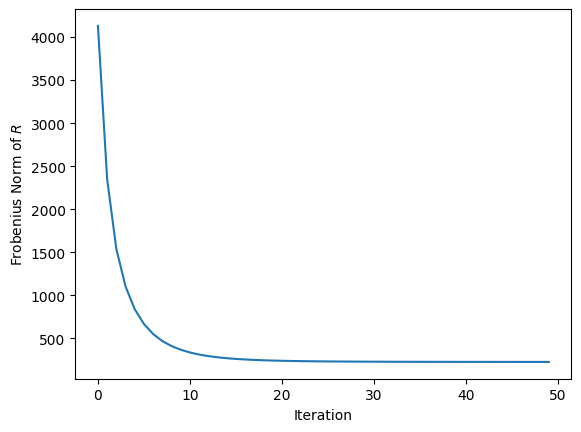
\includegraphics[scale=0.7]{pgd.png}
      \end{center}
      We see that after around 20 iterations, the norm of the residual $\lVert R \rVert_F$ stops changing visibly. Running the code several times, the eventual norm does not appear to depend on the initial approximation.

      I hypothesize the common theme of these documents is that they are letters, hence words such as ``you'' and ``your'' corresponding to high numbers in the columns of $W$.
    \end{solution}
    \newpage
    \item Do the same task for the HALS algorithm (Section 5.3.2 in \texttt{LinearAlgebra.pdf}).
    \begin{solution}
      We produce the following plot for the HALS algorithm via \href{https://github.com/elijahkin/school/blob/main/umd/amsc660/hw6/hw6.ipynb}{this code}.
      \begin{center}
        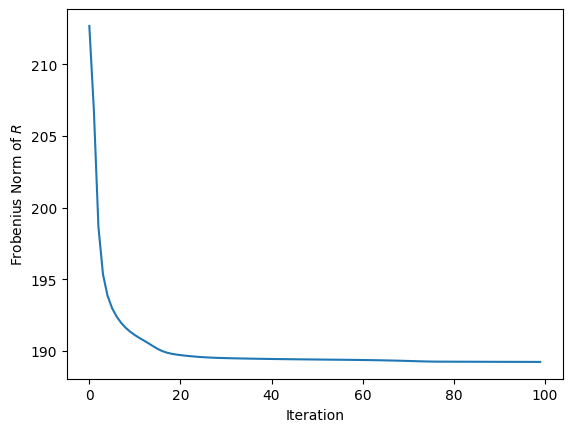
\includegraphics[scale=0.7]{hals.png}
      \end{center}
      We see that after around 30 iterations, the norm of the residual $\lVert R \rVert_F$ stops changing visibly. Running the code several times, the eventual norm does not appear to depend on the initial approximation.
    \end{solution}
    \item Find the best approximation $A_{10}$ of $A$ by a matrix of rank $\leq 10$ using SVD. Compute $\lVert A - A_{10} \rVert_F$. Compare it with the residuals.
    \begin{solution}
      After 50 iterations of projected gradient descent with a learning rate of $\alpha = 10^{-5}$, we achieve the final residual norm $\lVert R \rVert_F \approx 227.85$. Likewise, after 100 iterations of the HALS algorithm, we achieve the final residual norm $\lVert R \rVert_F \approx 189.22$.

      In contrast, taking the truncated SVD $A_{10}$ of $A$, we find that $\lVert A - A_{10} \rVert_F \approx 187.72$. Hence, we see that the HALS algorithm comes much closer to the norm of the best approximation of $A$ with $\operatorname{rank} \leq 10$.
    \end{solution}
  \end{enumerate}
\end{questions}

\end{document}
